\documentclass{book}
\usepackage[brazilian]{babel}
\usepackage[utf8]{inputenc}
\usepackage[T1]{fontenc}
\usepackage{multirow}

\usepackage{amsmath}
\usepackage{graphicx}
\graphicspath{ {Figures/} }
\usepackage{float}
\usepackage[dvipsnames]{xcolor}
\usepackage{tcolorbox}

\usepackage{natbib,stfloats}

\tcbuselibrary{skins,breakable}
\usetikzlibrary{shadings,shadows}
\usepackage{rotating}

\usepackage{tikz}
\usetikzlibrary{snakes}
\usetikzlibrary{patterns}

\usepackage{colortbl}
\newcolumntype{a}{>{\columncolor{yellow}}l}
\newcolumntype{b}{>{\columncolor{blue}}l}
\newcolumntype{d}{>{\columncolor{green}}l}

\usepackage{pdfpages}

\usepackage{fancyhdr}
\pagestyle{fancy}

\fancyhead{}
\fancyhead[RO]{\textsl{\rightmark}} 
\fancyhead[LE]{\textsl{\leftmark}} 

\fancyfoot{} 
\fancyfoot[L]{T.B. Fraga. thoughts: possible solution to global warming.}
\fancyfoot[R]{\thepage}

\definecolor{cambridgeblue}{rgb}{0.64, 0.76, 0.68}
\definecolor{camel}{rgb}{0.76, 0.6, 0.42}
\definecolor{camouflagegreen}{rgb}{0.47, 0.53, 0.42}
\definecolor{desertsand}{rgb}{0.93, 0.79, 0.69}

\newenvironment{exerciseblock}[1]{%
    \tcolorbox[beamer,%
    noparskip,breakable,
    colback=camel!20,colframe=camouflagegreen,%
    colbacklower=camouflagegreen!75!camel!20,%
    title=#1]}%
    {\endtcolorbox}

\newenvironment{exempleblock}[1]{%
    \tcolorbox[beamer,%
    noparskip,breakable,
    colback=camel!20,colframe=Brown!70,%
    colbacklower=camouflagegreen!75!camel!20,%
    title=#1]}%
    {\endtcolorbox}

\newenvironment{algorithmblock}[1]{%
    \tcolorbox[beamer,%
    noparskip,breakable,
    colback=camel!20,colframe=Brown!40,%
    colbacklower=camouflagegreen!75!camel!20,%
    title=#1]}%
    {\endtcolorbox}

\newenvironment{dedication}
  {\clearpage           % we want a new page
   \thispagestyle{empty}% no header and footer
   \vspace*{\stretch{1}}% some space at the top 
   \itshape             % the text is in italics
   \raggedleft          % flush to the right margin
  }
  {\par % end the paragraph
   \vspace{\stretch{3}} % space at bottom is three times that at the top
   \clearpage           % finish off the page
  }

% para construção de diagramas

\tikzstyle{place}=[circle,draw=camouflagegreen!80,fill=desertsand!20,thick]
\tikzstyle{Ret}=[rectangle,draw=camouflagegreen!80,fill=desertsand!20,thick]
\tikzstyle{RoundRet}=[rectangle,draw=camouflagegreen!80,fill=desertsand!20,thick, rounded corners]

\begin{document}

I am a scientist and true scientists are first and foremost great observers. It's been a few years since I've observed something interesting. \\

Some places on our planet have a unique property. Influence on the climate. Through observations and old memories, I realized that maybe it is possible to cause rain, just by heating some special environments with a big bonfire. \\

In the place where I live, I observed that people set fire to the dry forest, and approximately two days later, the rains start. This is interesting. But it is only empirical knowledge. \\

I believe that an in-depth study will show that in many cultures rituals were performed to bring about the rains. I believe that an in-depth study is warranted on whether ancient and current rituals hold ancient and extremely relevant knowledge.\\

Perhaps this knowledge can help control the planet's temperature. I hope so.

... \\

Let's include some experimental data... \\


weather forecast - PE on 11/27/2022 for the next fifteen days:

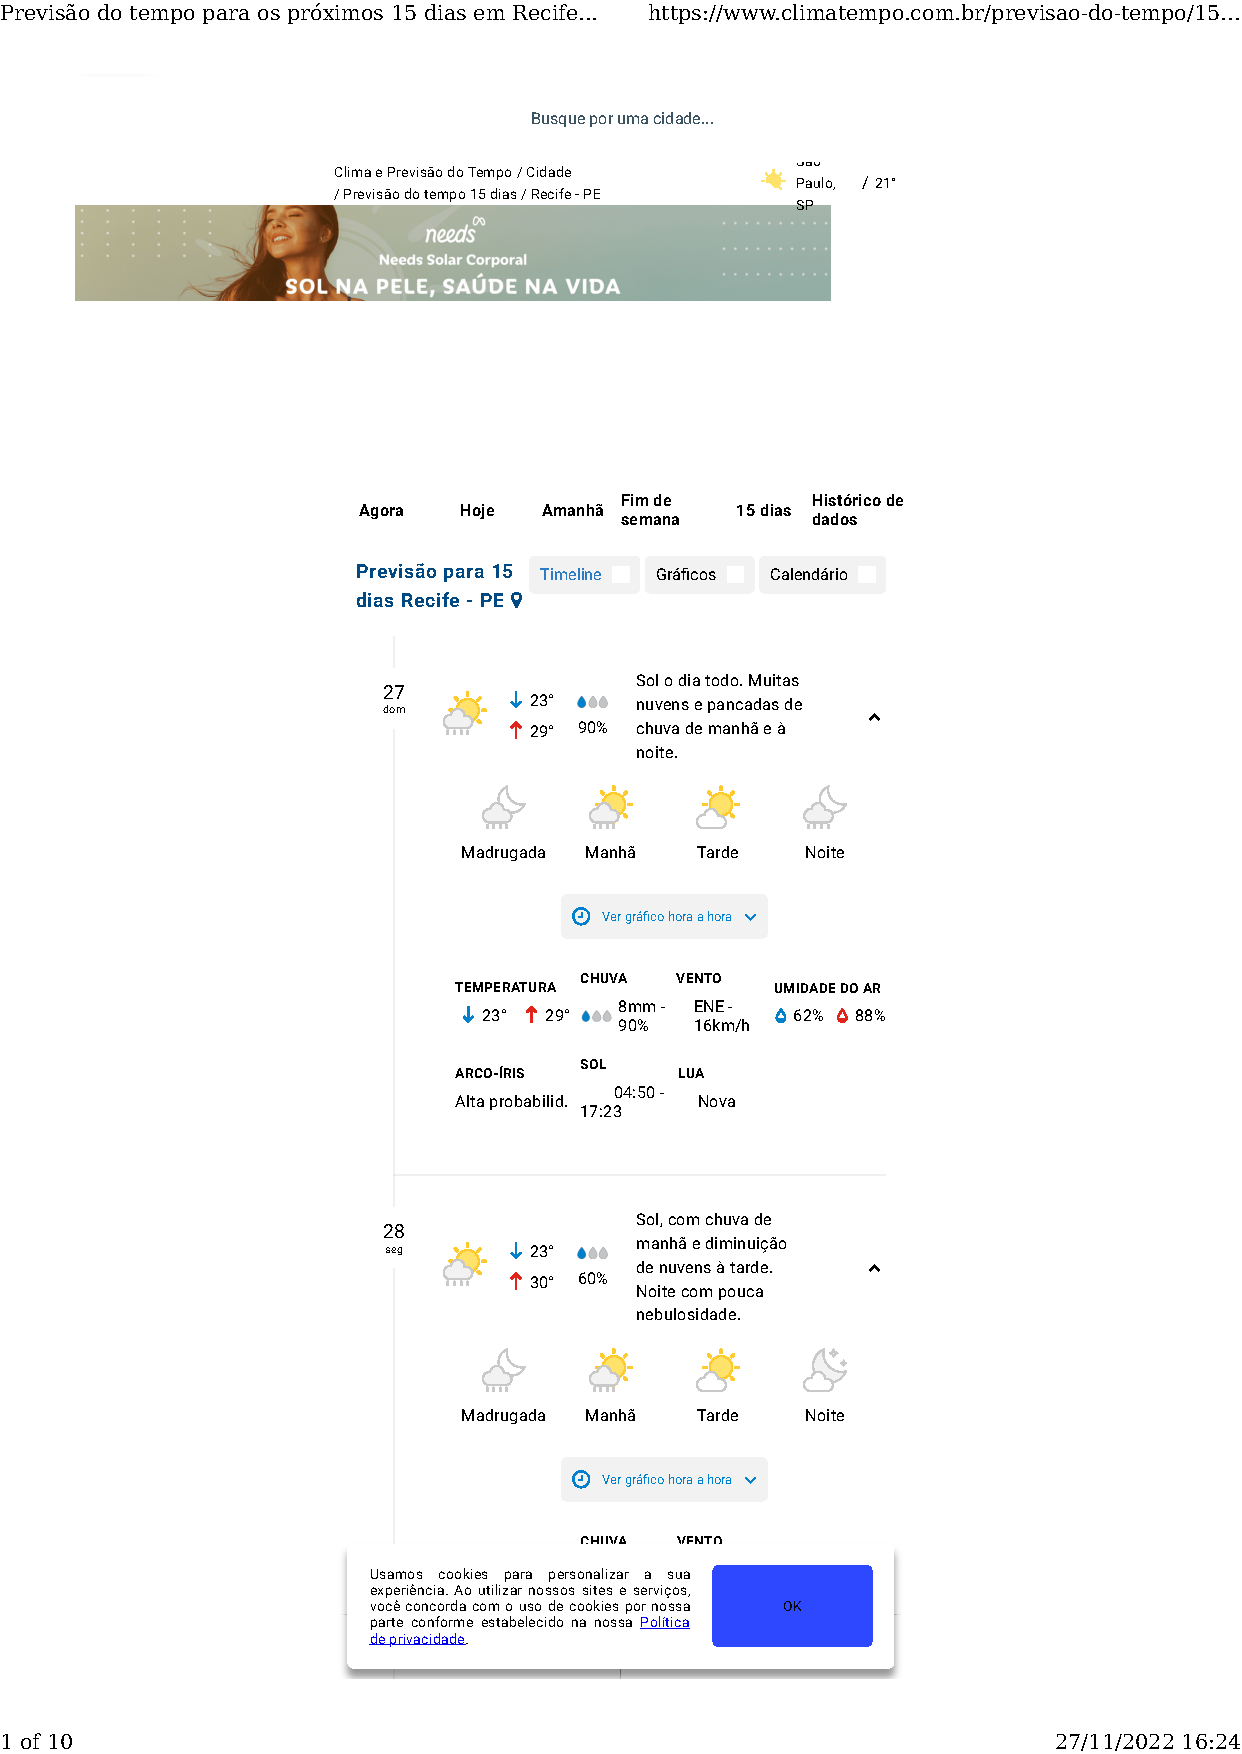
\includepdf[pages={1-6}]{figures/prediction.pdf}

\begin{figure}[h]
	\begin{center}
	    \caption{Photo after burning the bush near my house on 2022/12/01, Chã Grande - PE - Brazil.}
		\label{fig:bushBurning}
		\centering
		\includegraphics[width=\textwidth]{figures/IMG_20221201_142418.jpg}
	\end{center}
\end{figure}

\begin{figure}[h]
	\begin{center}
	    \caption{Rain all day on 2022/12/05, Chã Grande - PE - Brazil.}
		\label{fig:rain1}
		\centering
		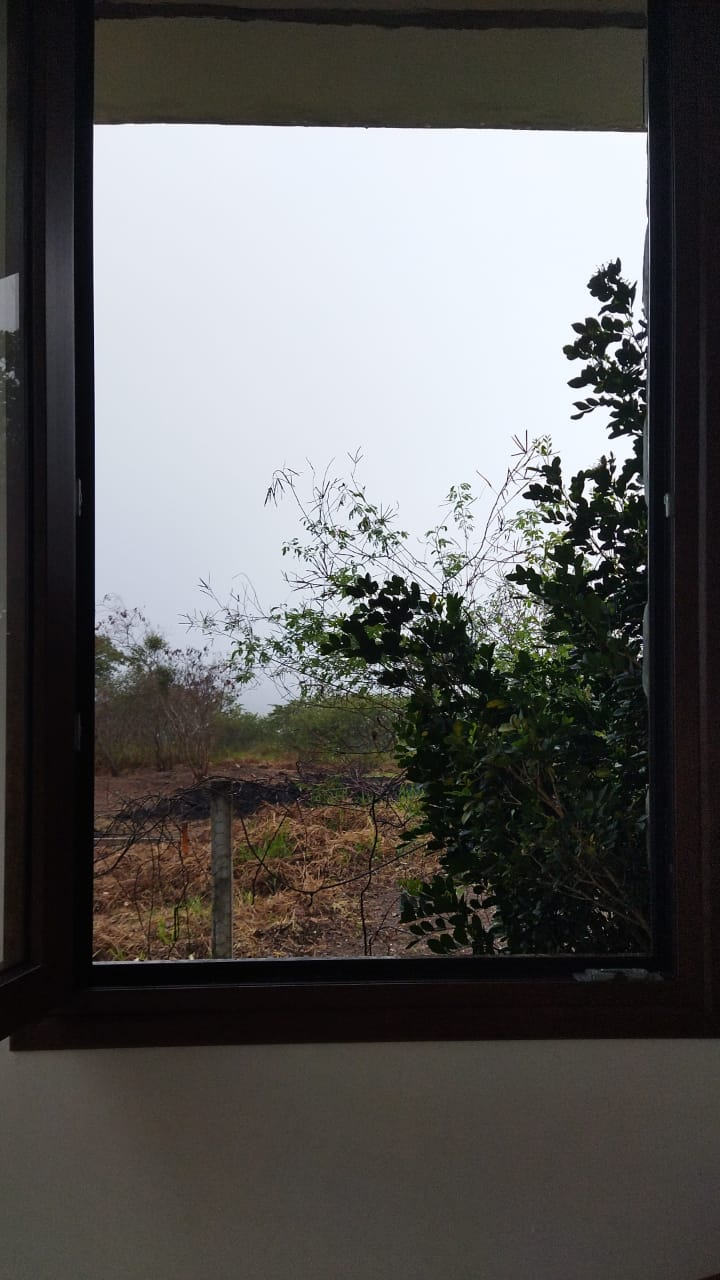
\includegraphics[width=\textwidth]{figures/IMG-20221205-WA0005.jpg}
	\end{center}
\end{figure}

\begin{figure}[h]
	\begin{center}
	    \caption{Rain all day on 2022/12/05, Chã Grande - PE - Brazil.}
		\label{fig:rain2}
		\centering
		\includegraphics[width=\textwidth]{figures/IMG_20221205_171659.jpg}
	\end{center}
\end{figure}

\end{document}
